\documentclass{scrartcl}
\usepackage[utf8]{inputenc}
\usepackage[english]{babel}
\usepackage{caption}
\usepackage{subcaption}
\usepackage{listings}
\usepackage{pdfpages}
\usepackage{amsmath,amssymb}
\usepackage{siunitx}
\usepackage{hyperref}
\usepackage{mhchem}
\usepackage[section]{placeins}
\usepackage[activate, protrusion=true, expansion=true]{microtype}
\usepackage[left=2.5cm, right=2.5cm, bottom=2.5cm, top=2.5cm]{geometry}
\usepackage{libertine}
\usepackage{longtable}

\lstset{frame=single,keepspaces=true,captionpos=b}

\title{System Identification (ME421) at EPFL}
\subtitle{CE-1: Nonparametric Methods}
\author{\textsc{Julia Krottenthaler} \and \textsc{Arne Sachtler}}
\date{\today}

\begin{document}
\maketitle

\section{Step Response}

Figure~\ref{fig:testmodel} shows the modelled system, which will be used for the system identification exercises.
\textcolor{red}{TODO: is this a reasonable choice question}
Figure~\ref{fig:responses} shows the step and impulse response for the system. On the left hand side the noise is included, the right hand side shows the responses without noise.

\begin{figure}[h]
	\centering
	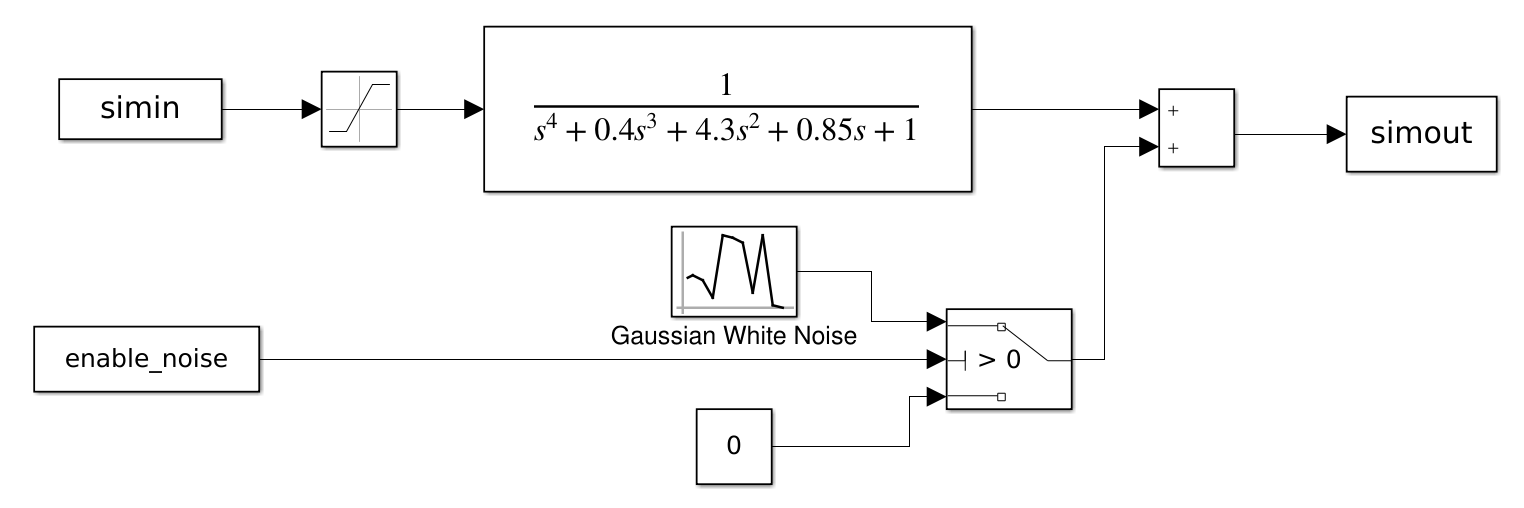
\includegraphics[height=4cm]{figures/systemmodel.png}
	\caption{Simulink model of the test system}\label{fig:testmodel}
\end{figure}


\begin{figure}[h]
	\centering
	\begin{subfigure}{0.49\textwidth}
		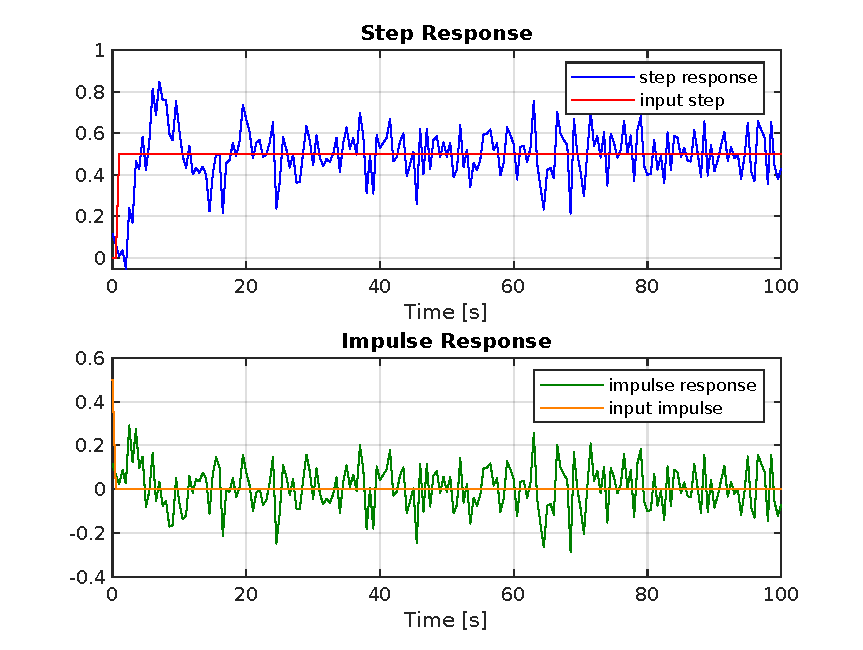
\includegraphics[width=\textwidth]{figures/noisy_responses.pdf}
		\subcaption{Noisy responses}
	\end{subfigure}
	\begin{subfigure}{0.49\textwidth}
		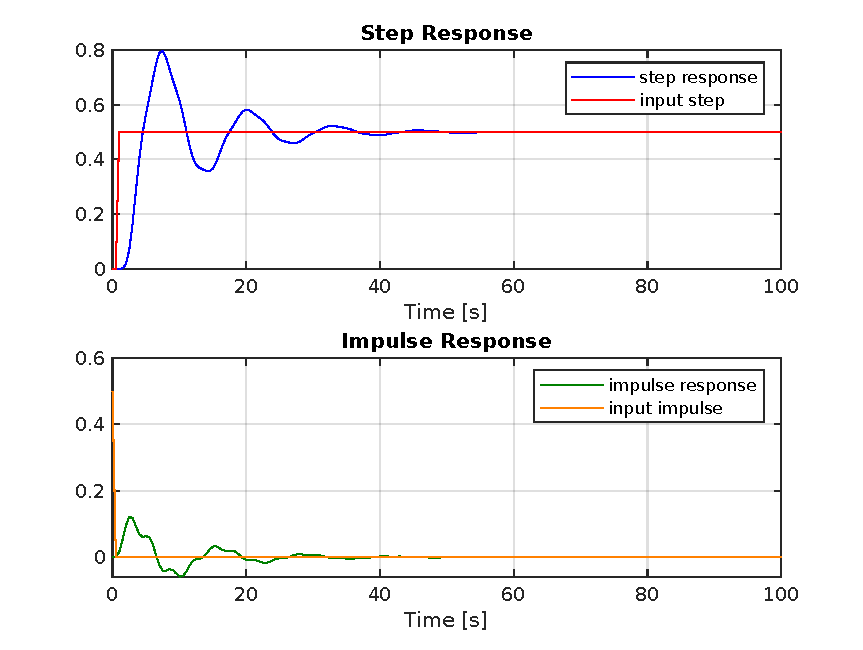
\includegraphics[width=\textwidth]{figures/noisefree.pdf}
		\subcaption{Responses without noise}
	\end{subfigure}
	\caption{Step and impulse responses of the test system with and without noise.}\label{fig:responses}
\end{figure}

\newpage

\section{Auto Correlation of a PRBS signal}

Figure~\ref{fig:autocorr} shows the autocorrelation function of two different types of signals. 
On the left hand side (Figure~\ref{fig:autocorrPRBS}) there is a PRBS signal (length of the shift register is 4 and number of periods is 2) and its corresponding autocorrelation function. 
In addition, the figure on the right hand side (Figure~\ref{fig:autocorrSINUS}) displays a sinusiodal signal and its autocorrelation function.  

\begin{figure}[h]
	\centering
	\begin{subfigure}{0.49\textwidth}
		\includegraphics[width=\textwidth]{figures/Autocorrelation_PBRS.png}
		\subcaption{PRBS signal}
		\label{fig:autocorrPRBS}
	\end{subfigure}
	\begin{subfigure}{0.49\textwidth}
		\includegraphics[width=\textwidth]{figures/Autocorrelation_Sinus.png}
		\subcaption{Sinus signal}
		\label{fig:autocorrSINUS}
	\end{subfigure}
	\caption{Two signals and their corresponding autocorrelation function}\label{fig:autocorr}
\end{figure}


\end{document}
